\section{Independent Forest Updates and Binding Constraints}\label{app:forest}
\subsection{Complete prespecified grid}
The protocol fixes three datasets, twenty seeds 20261108--20261127,
four nested feature counts $m\in\{3,6,9,12\}$ and cap three. WDBC uses
100 old-training, 200 new-training and 269 evaluation records; Spambase
uses 500, 1,000 and 3,101; Ionosphere uses 60, 120 and 171. We binarize
strictly above pooled training medians. Among columns varying on these
training records, take twelve evenly spaced column indices, then the
first $m$. Feature selection does not inspect labels. Each version fits
twenty depth-three trees with bootstrap samples, square-root feature
sampling and minimum leaf size $\max(3,n_{\rm old}/30)$ rounded down.
The versions have separate training records and seeds. The target is
$Y(p_1-p_0)$ for probability averages; thresholding a forest may destroy
degree-three identification.

Training records also fit the reference marginals, with uniform shrinkage
0.1 and a design floor $q_\iota\ge0.05/|\A|$. These are records used to fit
the evaluated models, so their in-sample paired loss is not an independent
target audit. No fresh complete calibration sample is excluded from the
acquisition accounting. Exact variances below condition on the fitted
models, reference and empirical held-out law. Repeated splits reuse
records, and their quantiles describe the experiment rather than
independent population replications.

\begin{figure}[ht]
\centering
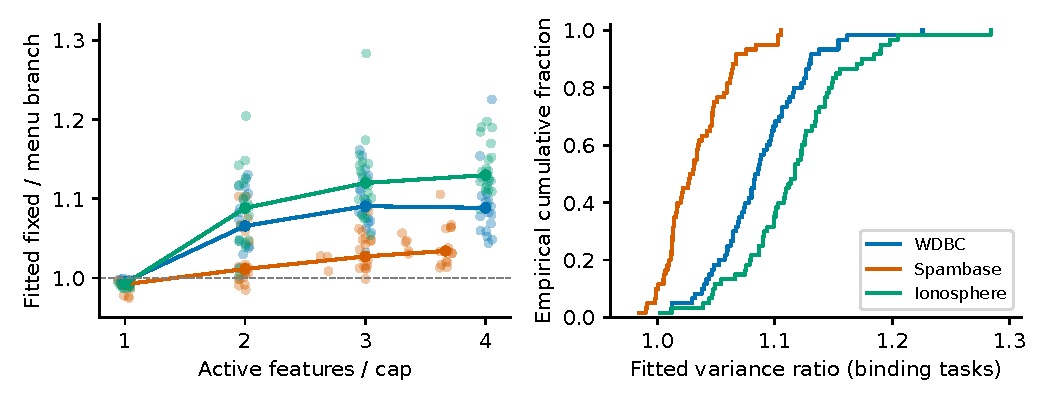
\includegraphics[width=.95\textwidth]{figures/forest_binding.pdf}
\caption{Every forest comparison and the distribution of the 180 binding
cases. Lines in the left panel join dataset medians across candidate
feature counts; models are refitted at each count, so the plot is not a
causal or monotonicity claim about active features. The right panel shows
the full empirical distribution.}
\label{fig:forestbinding}
\end{figure}

\subsection{Branching denominator and numerical bounds}
The fixed menu contains every size-three coordinate set. The tested
branch menu contains those forms and all forty component trees of the two
forests. Joint optimization uses the observed leaf, label and selected
tree, with the same pointwise target identity as fixed-form optimization.
It does not read all forest predictions on one person. We also implement
a centered random-component score: for signed forest weights $w_j$,
reference centers $\mu_j$, and $c=\sum_jw_j\mu_j$, return
\[
 H=Y\left(c+\frac{w_J\{f_J(X)-\mu_J\}}{q_J}\right).
\]
Reference residual second moments choose $q_J$, with the same 0.05 uniform
floor. The selected component's depth is at most three.

For each menu the reference-fitted procedure is evaluated on the held-out
law. Its ratio can be below one: fitting error and the menu-specific
positive probability floors can make the larger menu's implemented score
worse. This is not a reversal of the optimal information comparison.
Separate population-oracle programs omit the floor and jointly optimize
the design and all cell scores. Their primal values and dual witnesses
give numerical intervals, with explicit zero-mass-cell projections and
full-cube unbiasedness repair. These are floating-point checks, not exact
rational certificates. The maximum oracle ratio interval width is 0.00749;
the maximum score or zero-cell residual is $2.3\times10^{-15}$.

Let $W_F$ denote the unrestricted fixed-form optimum and $W_M$ the optimum
of the supplied branch menu. Since the menu is feasible,
$W_{\rm branch}\le W_M$, so $W_F^L/W_M^U$ lower-bounds
$W_F/W_{\rm branch}$. In contrast $W_F^U/W_M^L$ is only an upper endpoint
for $W_F/W_M$. The full-information variance supplies a separate, typically
looser upper bound $W_F^U/\Var(Yd)$ for the unrestricted ratio. We do not
infer that every depth-three adaptive strategy is close to the fixed
optimum. None of the tested fitted ratios exceeds 1.5; their maximum is
1.284. The largest oracle-menu lower endpoint is 1.207.
Appendix~\ref{app:forestexact} computes $W_{\rm branch}$ over all
depth-three trees by certified column generation, on a full-support version
of the held-out law. The exact ratios have median 1.51 on the binding tasks,
so this supplied menu understates the intrinsic ratio substantially.

\begin{table}[ht]
\centering
\caption{Full independent-forest grid: each row contains 20 fixed splits. Fitted ratio quantiles describe variation across overlapping splits; they are not confidence intervals. Oracle intervals concern the specified branch menu.}
\label{tab:forestdetail}
\small
\begin{tabular}{llrrrrr}
\toprule
Data & $m$ & Active median & Fitted median & Fitted 10--90\% & Oracle lower & Oracle upper \\
\midrule
Ionosphere & 3 & 3 & 0.992 & [0.987, 0.995] & 1.0000 & 1.0000 \\
Ionosphere & 6 & 6 & 1.088 & [1.036, 1.143] & 1.0699 & 1.0707 \\
Ionosphere & 9 & 9 & 1.120 & [1.076, 1.158] & 1.0992 & 1.0994 \\
Ionosphere & 12 & 12 & 1.130 & [1.107, 1.190] & 1.1053 & 1.1058 \\
Spambase & 3 & 3 & 0.992 & [0.978, 0.995] & 1.0000 & 1.0000 \\
Spambase & 6 & 6 & 1.011 & [0.991, 1.078] & 1.0258 & 1.0258 \\
Spambase & 9 & 9 & 1.027 & [1.011, 1.059] & 1.0332 & 1.0335 \\
Spambase & 12 & 11 & 1.034 & [1.016, 1.064] & 1.0362 & 1.0364 \\
WDBC & 3 & 3 & 0.995 & [0.991, 0.998] & 1.0000 & 1.0000 \\
WDBC & 6 & 6 & 1.066 & [1.012, 1.117] & 1.0861 & 1.0878 \\
WDBC & 9 & 9 & 1.091 & [1.062, 1.139] & 1.0941 & 1.0976 \\
WDBC & 12 & 12 & 1.089 & [1.052, 1.133] & 1.0810 & 1.0845 \\
\bottomrule
\end{tabular}
\end{table}


\subsection{Structural ties in the independent-tree benchmark}\label{app:binding}
The eight-feature experiment in Appendix~\ref{app:medium} must be stratified
per task, rather than comparing separate medians of active feature count
and cap. Among probability-output contrasts, 39/45 SUSHI and 21/25 SAPA
tasks are binding. Within those strata, median population ratios are
1.353 and 1.295; median global ratios remain 1.000. The other ten tasks
have a form that computes their contrast exactly. Among 58 nonzero
thresholded contrasts, 35/39 SUSHI and 17/19 SAPA tasks are nonbinding.
The six binding threshold tasks have median population ratios 1.289 and
1.360 in the two datasets. Thus nonbinding budgets explain most
thresholded ties, not the probability-output results. The released
\texttt{independent\_binding\_strata.csv} contains every stratum.

